\chapter{Interfaccia Utente e Casi d'Uso}
Per validare il sistema di backend e le scelte descritte nei capitoli precedenti, è stato sviluppato un client web completo e responsivo tramite il framework Spring Boot. Di seguito vengono presentati i principali casi d'uso del sistema attraverso le interfacce utente dedicate ai vari ruoli.

\section{Accesso al Sistema}
La schermata di login rappresenta il singolo punto di ingresso per tutti gli utenti del sistema. Inserendo le proprie credenziali, la richiesta viene inviata al Server di Autenticazione. Una volta generato e validato il token di sessione, il sistema reindirizza automaticamente l'utente verso la dashboard dedicata al proprio ruolo.

\begin{figure}[h]
    \centering
    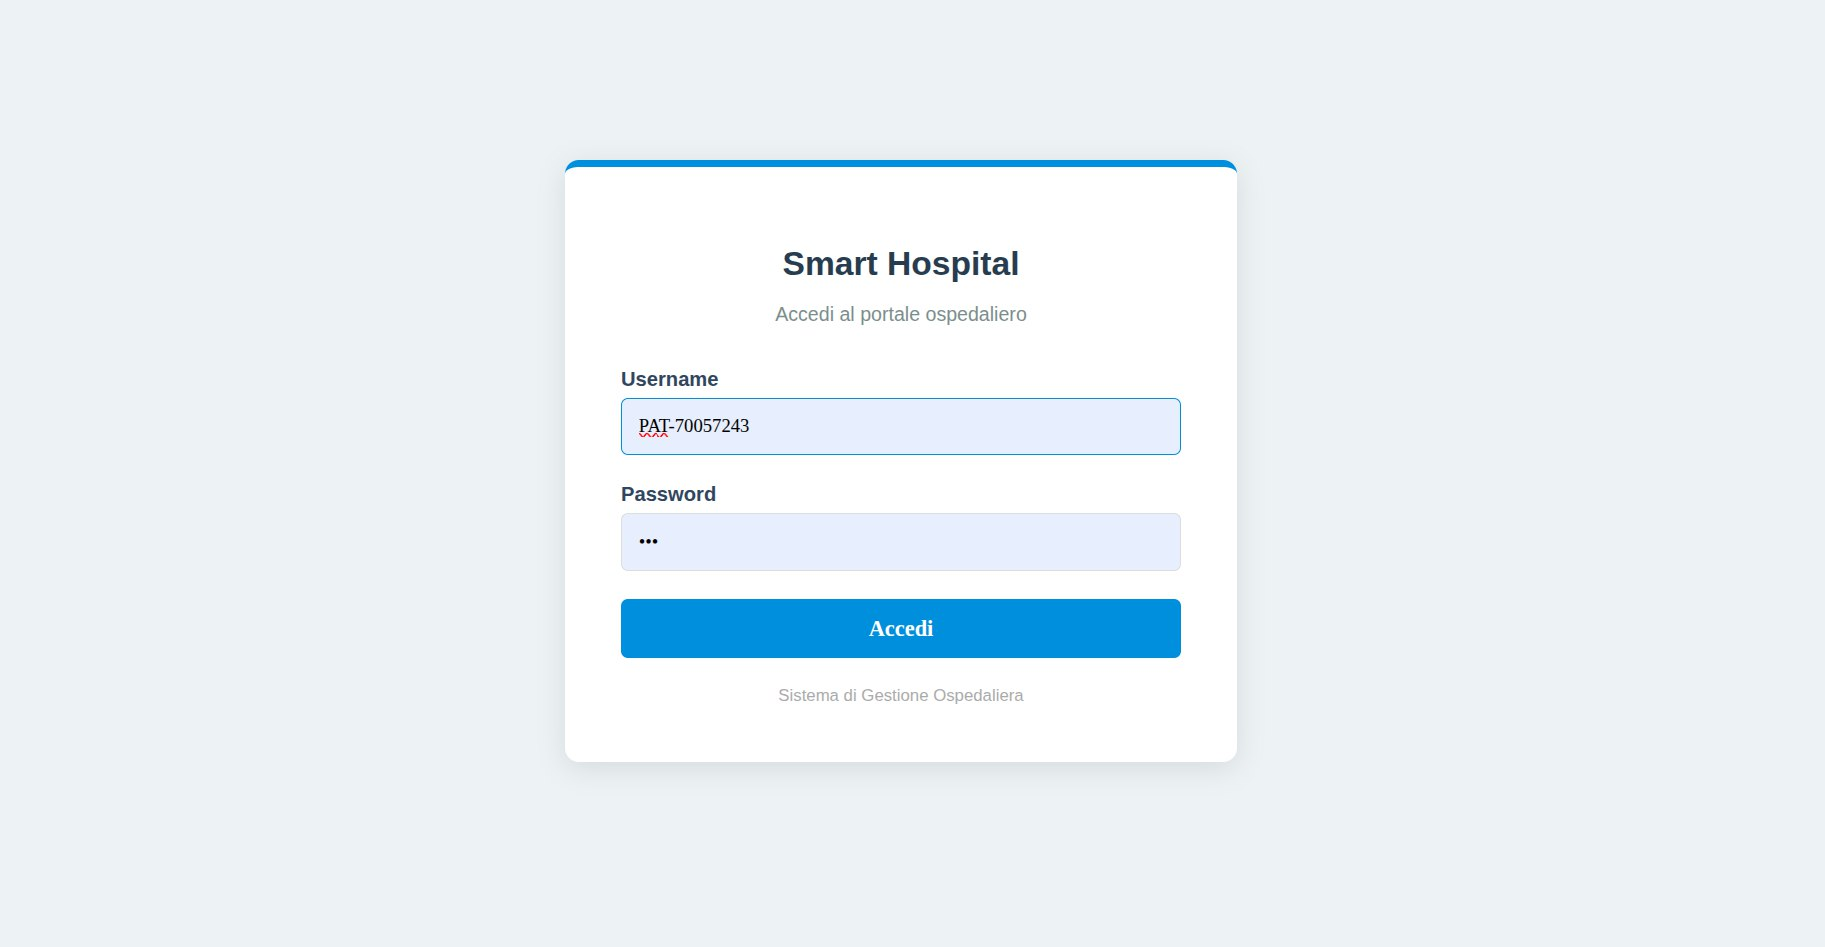
\includegraphics[width=0.7\textwidth]{Images/sito/Schermata_login.jpg} 
\end{figure}

Si segnala il fatto che, se l'utente prova ad andare alla schermata di login quando possiede ancora un token valido, allora questo viene indirizzato automaticamente alla dashboard bypassando il login.

\section{Dashboard Amministratore (Admin)}
L'interfaccia dedicata agli amministratori fornisce un pannello di controllo. Come si evince dall'interfaccia, l'amministratore ha a disposizione gli strumenti per monitorare in tempo reale le statistiche di occupazione dei reparti e analizzare i dati storici. 
\begin{figure}[h]
    \centering
    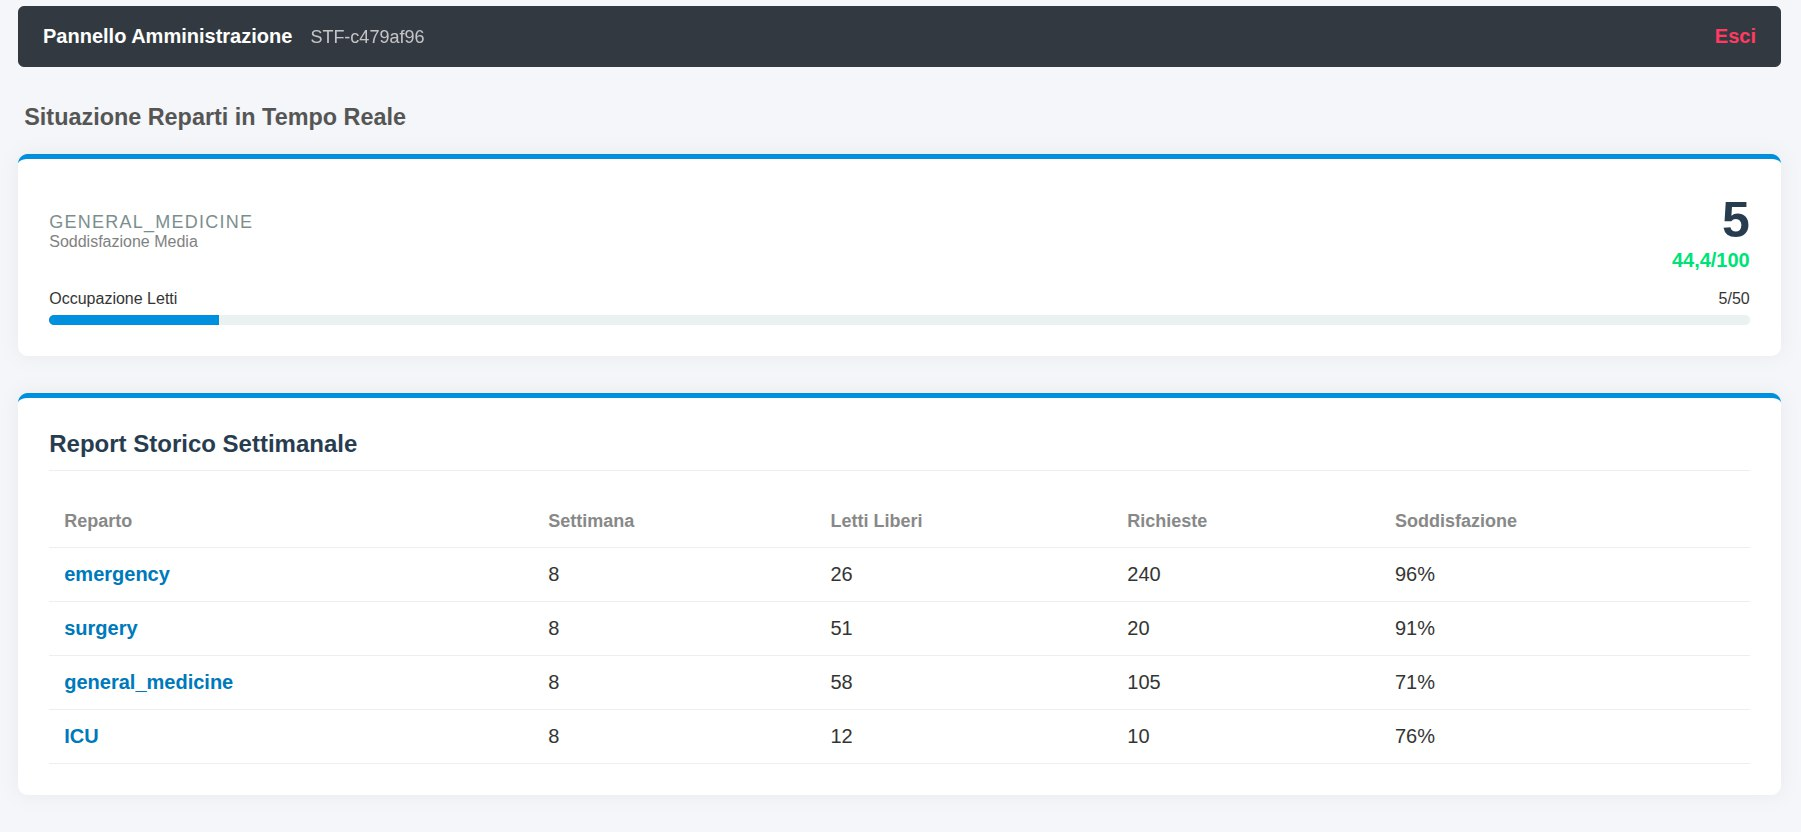
\includegraphics[width=0.85\textwidth]{Images/sito/Schermata_admin_1.jpg}
\end{figure}
Inoltre, la vista integra i form necessari per l'assunzione di nuovo personale e la registrazione di nuovi pazienti, interfacciandosi, in background, con l'\texttt{AdminService}.
\begin{figure}[h]
    \centering
    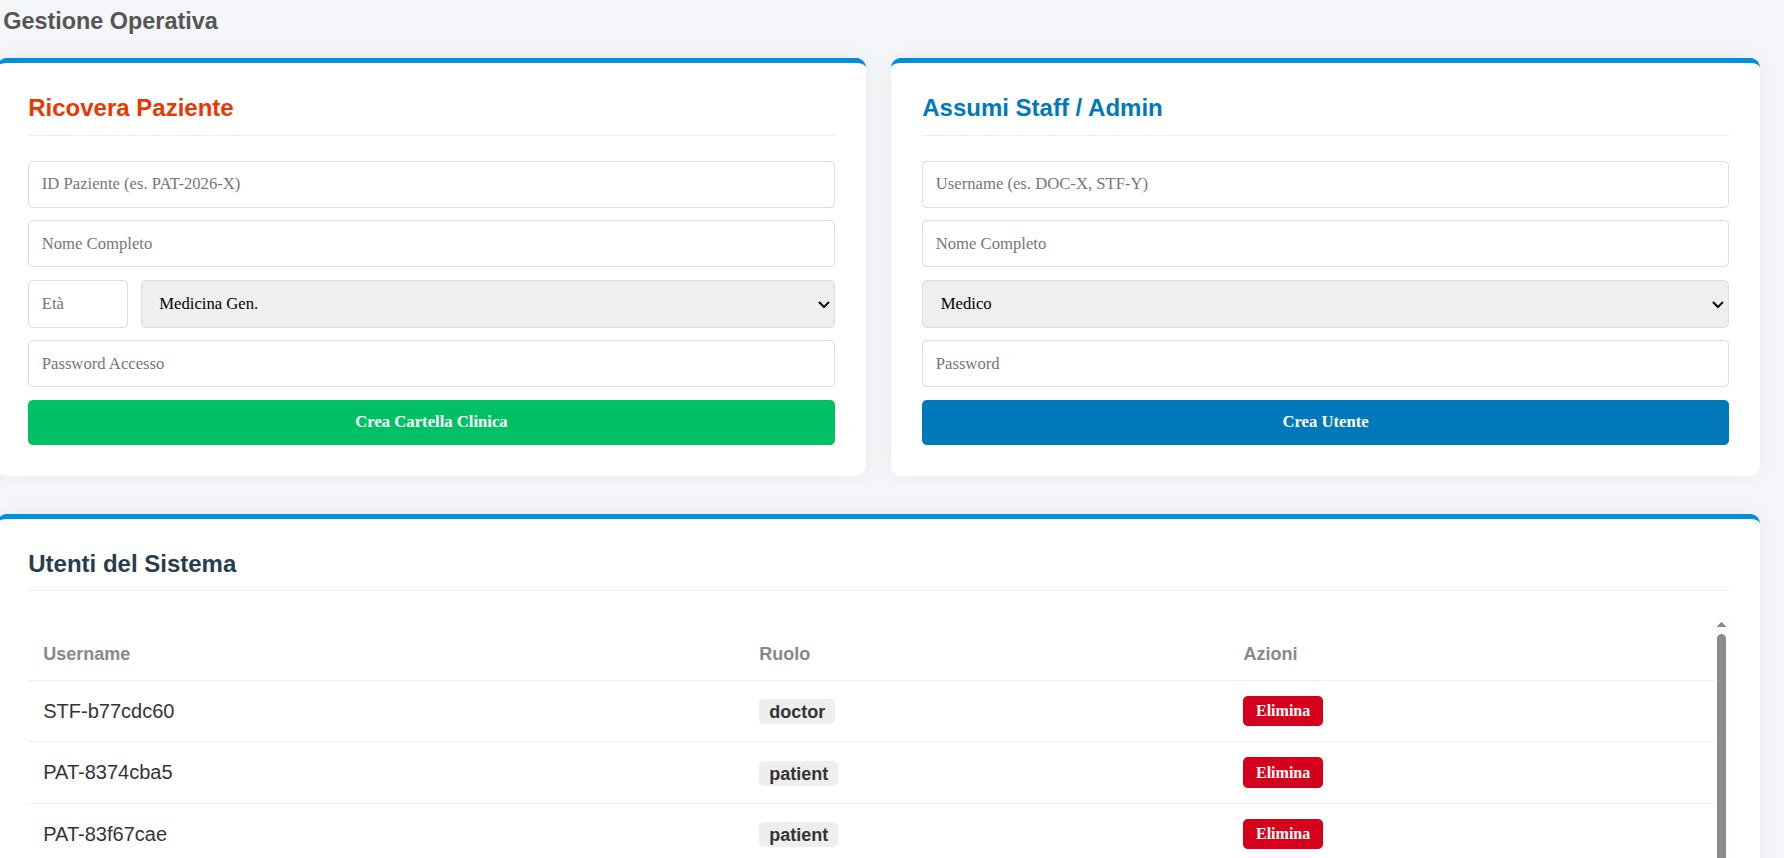
\includegraphics[width=0.85\textwidth]{Images/sito/Schermata_admin_2.jpg}
\end{figure}

\section{Dashboard Personale Sanitario (Staff)}
L'interfaccia per il personale medico (Doctor e Nurse) è progettata per ottimizzare la gestione del reparto. L'utente può visualizzare la lista dei pazienti attualmente assegnati al proprio reparto e consultare la propria turnazione lavorativa. 

\begin{figure}[h]
    \centering
    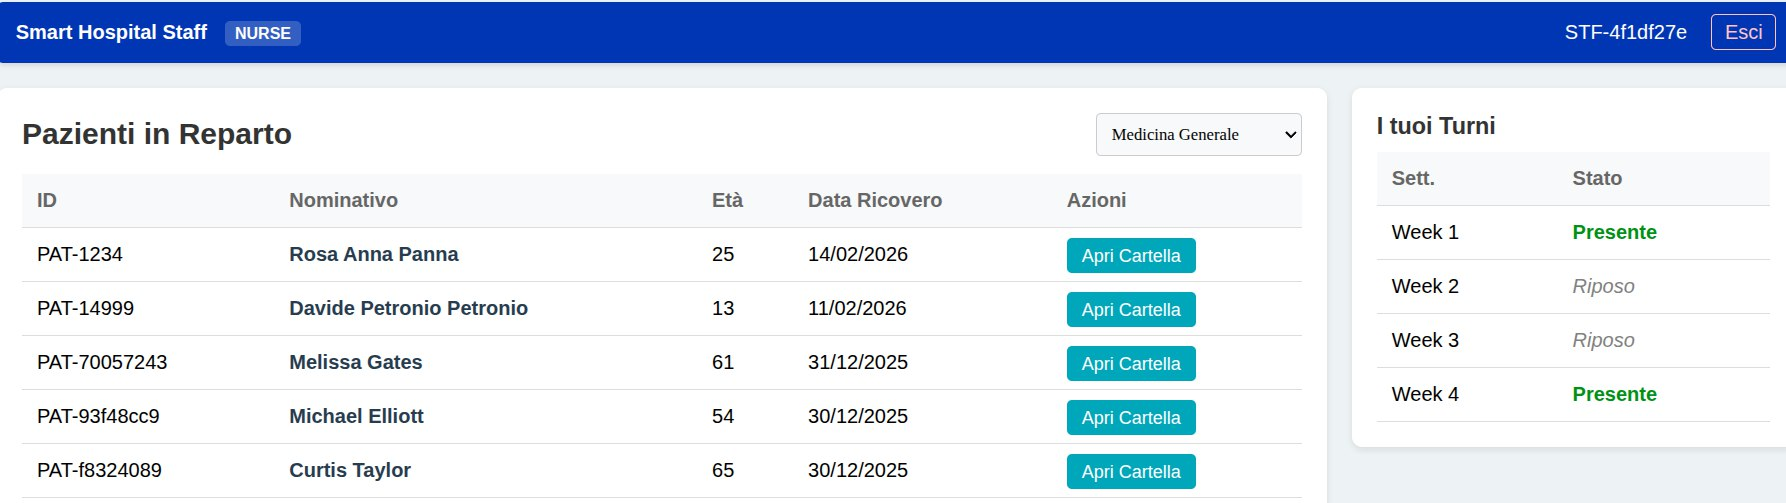
\includegraphics[width=0.85\textwidth]{Images/sito/Schermata_pazienti_infermiere.jpg}
\end{figure}


Entrando nel dettaglio di una cartella clinica, l'interfaccia si adatta dinamicamente alle policy RBAC descritte in precedenza: se l'utente è autenticato come medico , il frontend sblocca e mostra le azioni critiche come il form per prescrivere esami, aggiornare i referti e dimettere il paziente.

\begin{figure}[h]
    \centering
    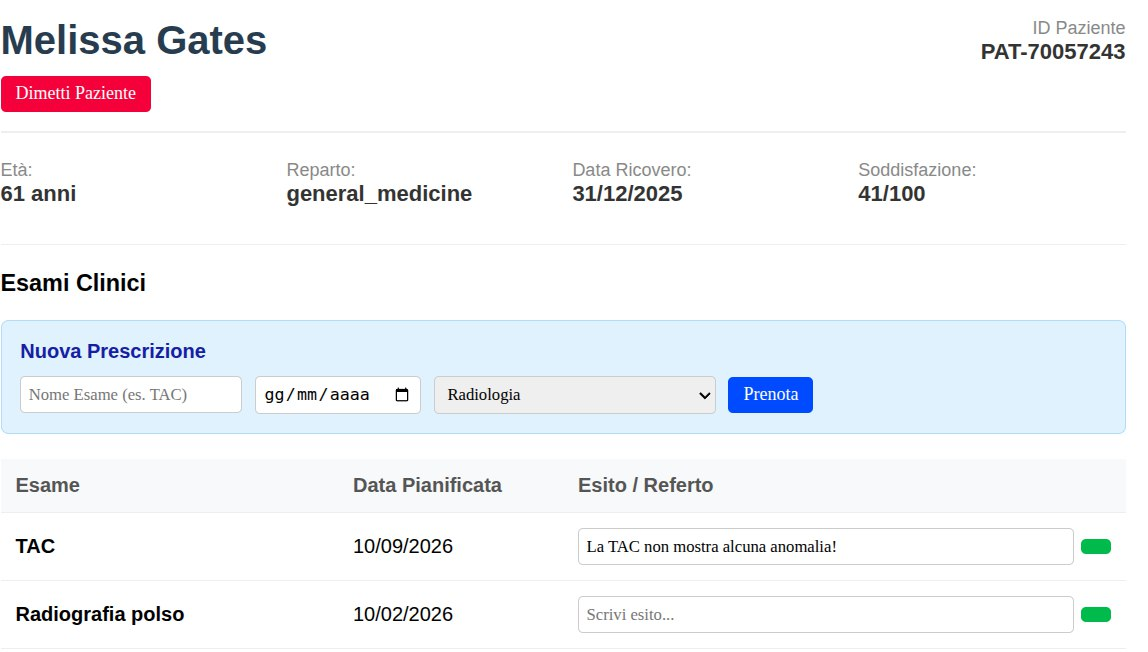
\includegraphics[width=0.85\textwidth]{Images/sito/Paziente_Dottore.jpg}
\end{figure}

Qualora l'accesso avvenga come infermiere, tali funzionalità non risultano presenti.

\begin{figure}[h]
    \centering
    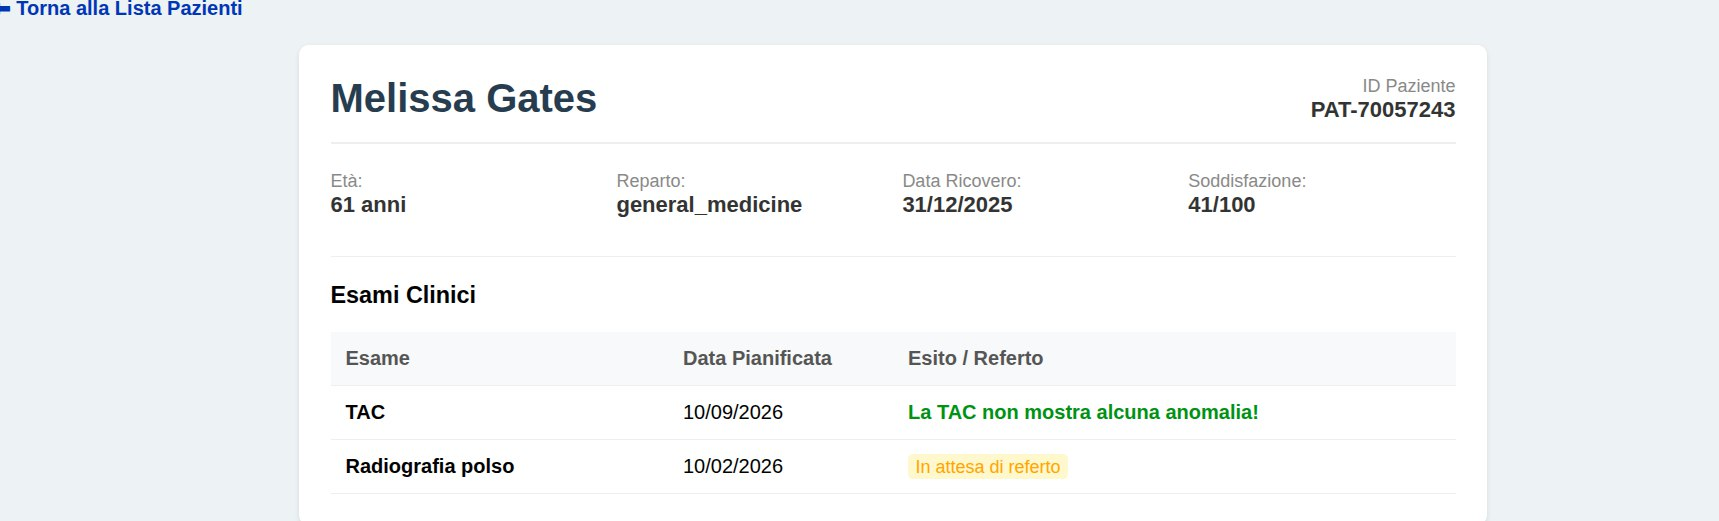
\includegraphics[width=0.85\textwidth]{Images/sito/Schermata_paziente_infermiere.jpg}
\end{figure}

\section{Portale Paziente}
Il paziente, una volta effettuato l'accesso, è in grado di visualizzare esclusivamente il riepilogo della propria cartella clinica personale e lo storico degli esami prescritti. Inoltre, l'interfaccia fornisce un modulo per inviare un feedback sul livello di soddisfazione delle cure ricevute, dato che andrà ad alimentare le statistiche di reparto gestite dal sistema.

\begin{figure}[h]
    \centering
    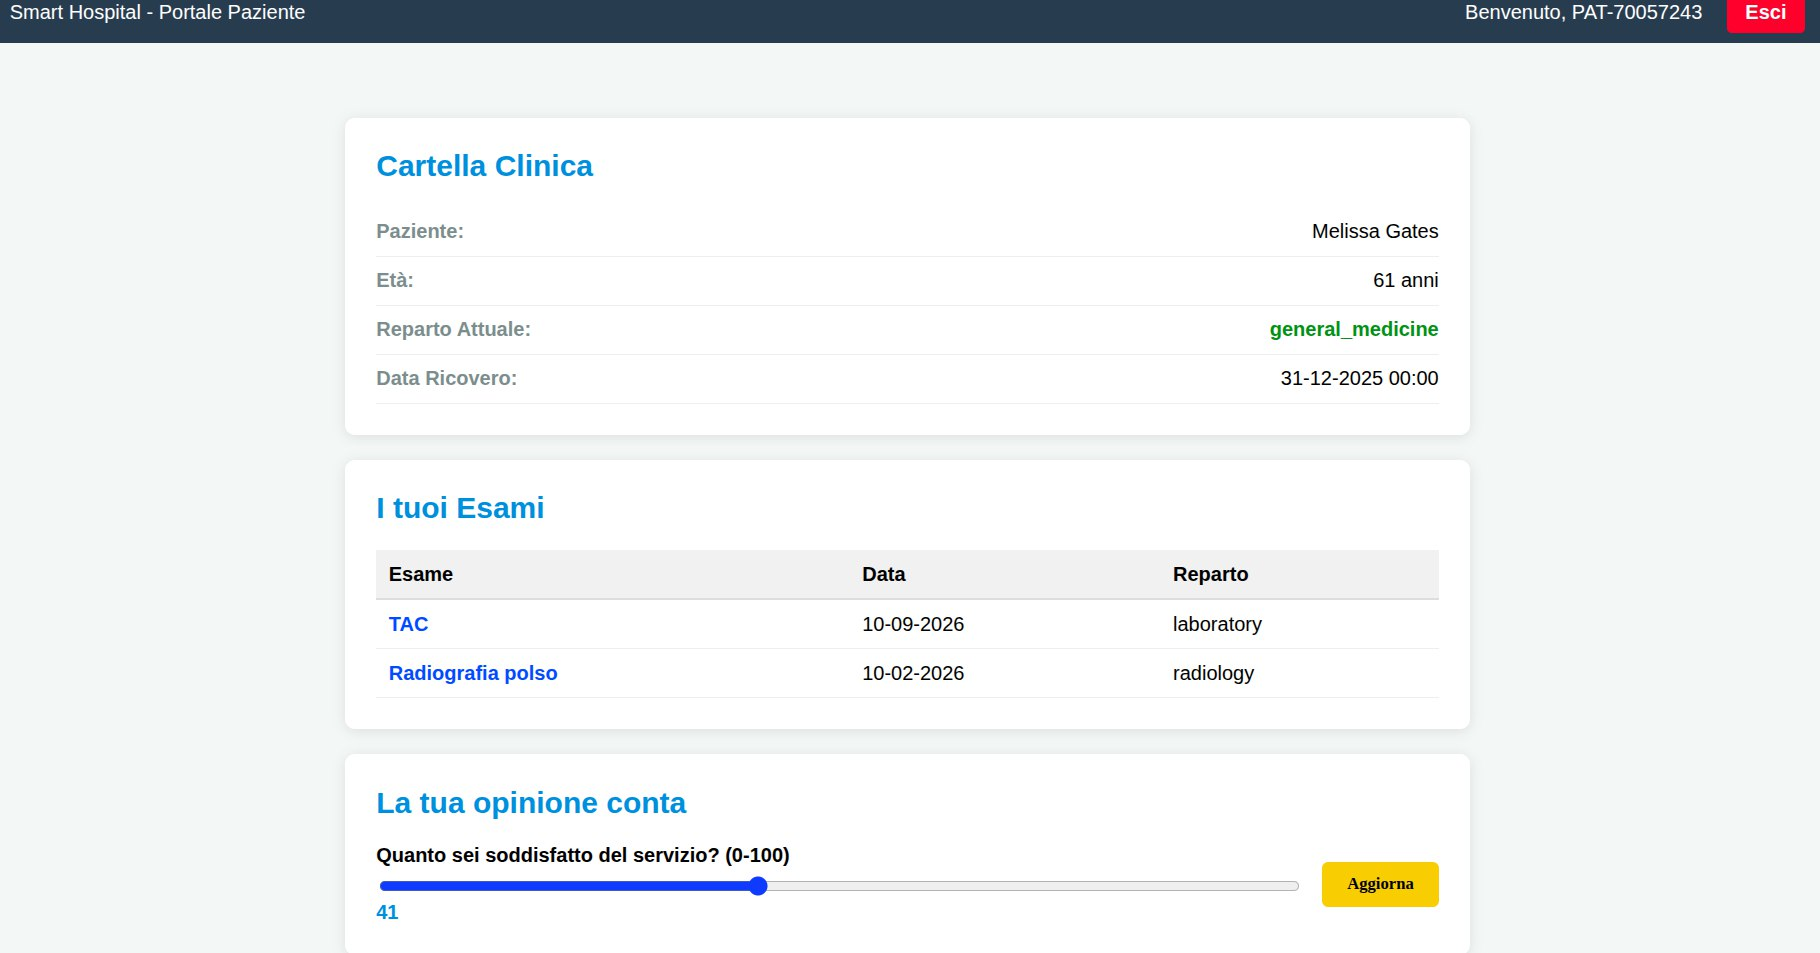
\includegraphics[width=0.85\textwidth]{Images/sito/Schermata_Paziente.jpg}
\end{figure}

Infine, è possibile per il paziente visualizzare tutti i riepiloghi dei suoi esami nel dettaglio.

\begin{figure}[h]
    \centering
    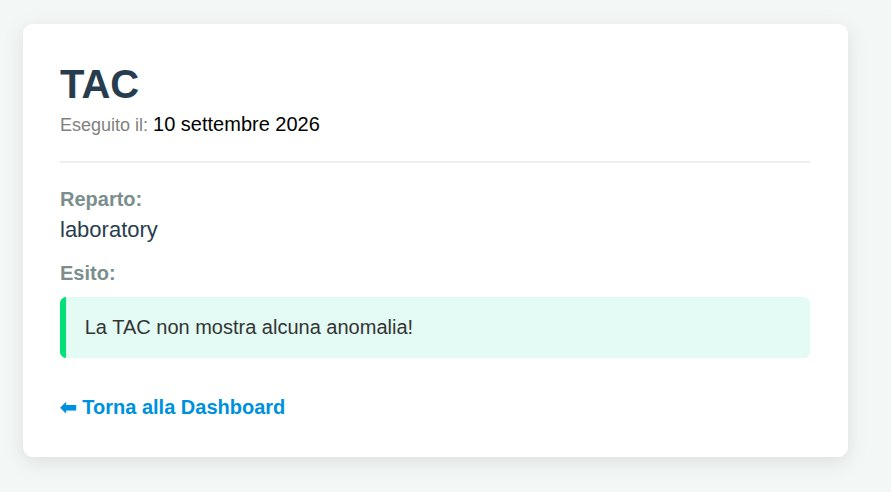
\includegraphics[width=0.85\textwidth]{Images/sito/Esame_Paziente.jpg}
\end{figure}
